% Created 2023-09-17 Sun 22:26
% Intended LaTeX compiler: pdflatex
\documentclass[12pt, a4paper]{article}
\usepackage[utf8]{inputenc}
\usepackage[T1]{fontenc}
\usepackage{graphicx}
\usepackage{longtable}
\usepackage{wrapfig}
\usepackage{rotating}
\usepackage[normalem]{ulem}
\usepackage{amsmath}
\usepackage{amssymb}
\usepackage{capt-of}
\usepackage{hyperref}
\usepackage{placeins}
\usepackage{gensymb}
\usepackage[letterpaper]{geometry}
\geometry{top=1.0in, bottom=1.0in, left=1.0in, right=1.0in}
\usepackage{rotating}
\usepackage{graphicx}
\usepackage{pgfplots}
\usepackage{filecontents}
\usepackage{tikz}
\usepackage{fancyhdr}
\pagestyle{fancy}
\lhead{}
\chead{}
\rhead{Johnson \thepage}
\lfoot{}
\cfoot{}
\rfoot{}
\renewcommand{\headrulewidth}{0pt}
\renewcommand{\footrulewidth}{0pt}
\setlength\headsep{0.333in}
\newcommand{\bibent}{\noindent \hangindent 40pt}
\newenvironment{workscited}{\newpage \begin{center} Works Cited \end{center}}{\newpage }
\graphicspath{ {./attachments/} }
\date{\today}
\title{}
\hypersetup{
 pdfauthor={},
 pdftitle={},
 pdfkeywords={},
 pdfsubject={},
 pdfcreator={Emacs 28.2.50 (Org mode 9.7-pre)}, 
 pdflang={English}}
\begin{document}

\begin{document}
\begin{flushleft}
Christian Johnson\\
\vspace{2mm}
Dr. Paul Crilly\\
\vspace{2mm}
Antennas and Propogation\\
\vspace{2mm}
September 16 2023\\
\vspace{4mm}
\begin{center}
Lab 1 Report
\end{center}
\vspace{1mm}
\setlength{\parindent}{0.5in}

\begin{abstract}

In this lab exercise, we explored the practical application of loop antennas and their application to signal location. The primary direction of this exercise was to locate the WXLM (980 kHz) radio station using our antenna to triangulate the approximate geographical location of the stations source. This involved constructing a parallel RLC circuit and manipulating circuit components to observe resonant frequencies. We saw how parasitic capacitance impacted the performance of our circuit, shedding light on the real world application of the theory that we discussed in class. By conjoining our theoretical knowledge with hands on experimentation, this exercise provided valuable insight into the fundamental mechanics of radio signal propogation and direction finding. 

\end{abstract}
\section*{Procedures}
\label{sec:orgb97c6c8}
In the initial phase of this experiment, we set out to construct our antenna. We coiled a length of copper wire until we reached approximately 20 to 30 turns of wire. We attached this wire to a board, with a "gimmick capacitor" of about 5.0 picofarads connected to one of the loops leads. This capacitor consists of 2 1" pieces of wire twisted together.
With this simplistic circuit constructed, we used an oscilloscope and a 1 volt sine wave to find the frequency at which we elicit the maximum response. Starting at around 300 kHz, we swept the frequency up until we found the maximum response at 1232 kHz. Our primary objective was to achieve a maximum response near, but above, 980 kHz (this is so that the capacitor we introduce next will be able to effectively reduce the maximum response to 980 kHz).
After finding our maximum response, we went on to add a variable capacitor into the circuit. Using the oscilloscope, we adjusted the capacitors value to find the range of frequencies for which we find a maximum response, finding this range to be 745 kHz to 1080 kHz. Adjusting the capacitor one final time, we ensure that the circuits maximum response fell as close to 980 kHz as possible.
Next, we form another loop of wire, consisting of about 7-10 wraps, and affix that to the same board. This new loop is in parallel to the original, close, but not connected to the first loop. It serves as a transformer, to convert between the LC circuit and the spectrum analyzer that we will use when testing our antenna. 
Once our circuit is fully constructed, we are able to begin taking measurements. We used the 9912A Field-Fox Spectrum Analyzer, attaching the leads from the second, smaller wire loop to the leads on the field-fox. In order to get the most accurate results possible, we chose 3 locations across campus, each as far apart as possible with a relatively unobstructed view across the river. At each location, we varied the orientation of the antenna. The field-fox generated an amplitude graph, and our goal was to analyze this graph to find the antenna orientation that gave us a minimum value. We then used a compass and a GPS to record our geographical coordinates, and the antennas angle in relation to true north. With this data, we were able to check the angles emanating from each of the three points to approximate a point of origin for the local 980 kHz radio station. 
\section*{Results}
\label{sec:org75eaa2e}
Over the course of our experiment, we successfully recorded coordinates and vectors at three points across campus. We took measurements at Cadet Memorial Field (CMF), Waterfront (WF) and the Rugby Field, included below.

\begin{table}[h]
\centering
\begin{tabular}{|c|c|c|c|}
\hline
Location & Latitude & Longitude & Angle (True) \\
\hline
CMF & N 41° 22' 20.85'' & W 72° 5' 58.38'' & 69.0° \\
Waterfront & N 41° 22' 29.79'' & W 72° 5' 49.09'' & 94.1° \\
Rugby Field & N 41° 22' 14.77'' & W 72° 5' 49.95'' & 63.7° \\
\hline
\end{tabular}
\caption{Coordinates and Angle Vectors for Various Locations}
\end{table}

It's important to note that the measurement we took at Waterfront appeared to deviate significantly from the data taken at CMF and the Rugby Field. We were forced to discard this data point, as the results it provided were not consistent with our other data or the result we expected to receive. Upon closer examination, we observed the two remaining data points to converge at a point of (41.381, -72.0699). This seems relatively accurate, as our expected location was (41.384722, -72.070278), which means that our result was only about 0.26 miles from the expected result. Our percent error in latitude was 0.009\%, and in latitude only 0.0005\%, for an average percentage error of 0.0045\%. 
\section*{Conclusions}
\label{sec:org14ff598}
In this lab exercise, we undertook a comprehensive exercise to explore radio direction finding using loop antennas. Using LC circuits, we sought to locate to origin point for the local radio station WXLM (980 kHz). Throughout this experiment we were able to record two relatively accurate data points and one outlier, resulting in an average percent error of 0.0045\%. Our data was somewhat surprising; given the relative inaccuracy of the equipment we used, we did not expect to receive such an accurate answer. In conclusion, this exercise helped to facilitate the practical application of theoretical knowledge, while exploring the basics of signal propagation and real-world electrical circuits. 

\newpage
\begin{center}
Apendices
\end{center}
\begin{figure}[htb]
\centering
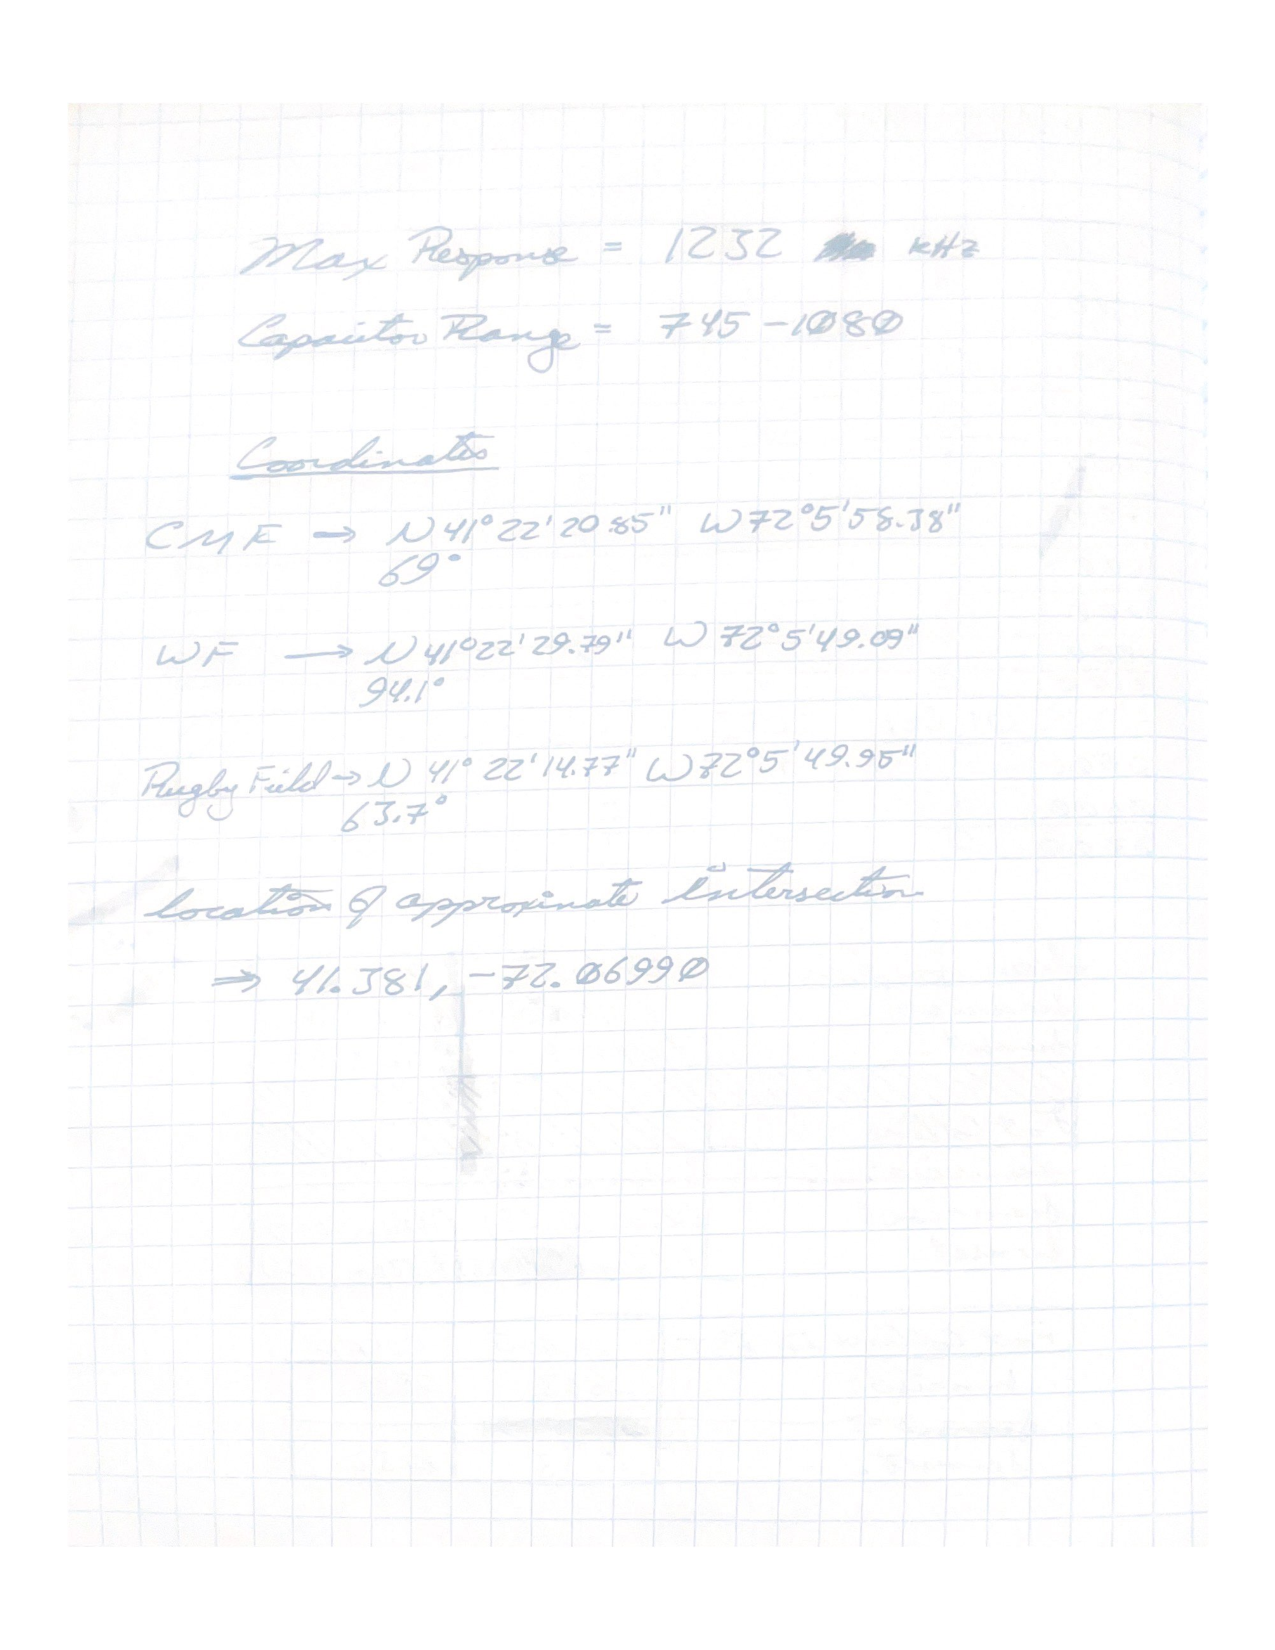
\includegraphics[width=0.7\textwidth]{Lab1-Data.pdf}
\caption{Recorded Data}
\end{figure}
\newpage
\begin{figure}[htb]
\centering
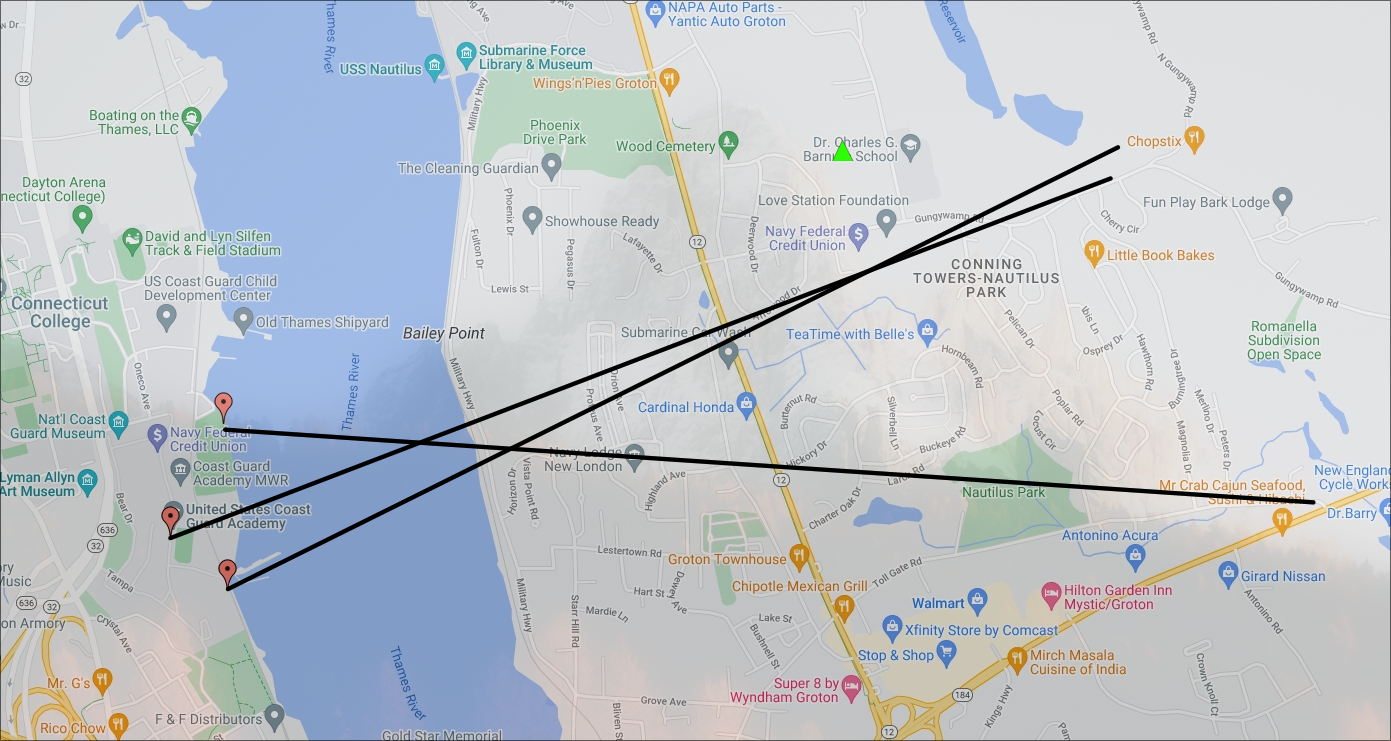
\includegraphics[width=0.6\textwidth]{Triangulation.png}
\caption{GPS data and Vectors}
\end{figure}
\newpage


\newpage
\begin{center}
Lab Questions
\end{center}

\begin{enumerate}

\item{Minimum lead length to create a parasitic resistance at (a) 1MHz (b) 10MHz (c) 100MHz (d) 1GHz}
\begin{itemize}
\item{\lambda = \frac{3*10^{8}}{1MHz} = 299.79 m\text{ Minimum Lead Length} \approx 0.01\text{ to }0.1\lambda\therefore\text{Minimum}\approx 2.99m}

\item{\lambda = \frac{3*10^8}{10MHz} = 29.979 m\text{ Minimum Lead Length}\approx0.01\text{ to }0.1\lambda\therefore\text{Minimum}\approx0.299m}

\item{\lambda = \frac{3*10^8}{100MHz} = 2.9979 m\text{ Minimum Lead Length}\approx0.01\text{ to }0.1\lambda\therefore\text{Minimum}\approx0.0299}

\item{\lambda = \frac{3*10^8}{1GHz} = 0.299 m\text{ Minimum Lead Length}\approx0.01\text{ to }0.1\lambda\therefore\text{Minimum}\approx0.00299}

\end{itemize}

\item{C_{p} = 250pf; L=126\mu H; C_{b}=50pf}

\begin{itemize}

\item Resonant Frequency = $103.84 MHz$

\item Resonant Frequency = ${\frac{1}{2\pi\sqrt{(126*10^-6)(295*10^-12)}}} = 7.07 MHz$

\item Resonant Frequency = ${\frac{1}{2\pi\sqrt{(126*10^{-6})(305*10^{-12})}}} = 8.05GHz$

\end{itemize}$

\item Find the parasitic capacitance of the coil. $L = 126\mu H$\\
$f_{0} = \frac{1}{2\pi\sqrt{LC_{parasitic}}}$\\
Given the results from 2b - $f_0 = 7070000 Hz$\\
\therefore 7070000 = ${1}/{2\pi\sqrt{126*10^{-6}*C}}$ = $\frac{1}{2.51*10^{10}\pi^{2}}$

\item Why was the null position of the antenna used?
The null position was used because it provides a more accurate indication of the direction of the signal source. Using the maximum response would not provide as clear an indication of the signal's direction.

\item Derive the impedance for an RLC circuit\\
$Z=\frac{1}{\frac{1}{R}+\frac{1}{-2\pi fL}+2fC\pi}$

\item What is the value of a parallel RLC circuit when $\omega=\frac{1}{\sqrt{LC}}$\\
$Z = \frac{1}{\sqrt{\frac{1}{R^2}+LC}}



\end{enumerate}


\end{document}
\end{document}